\begin{figure}[t]
  \centering
  \begin{tikzpicture}
    \node[inner sep=0pt] (map) at (0, 0)
         {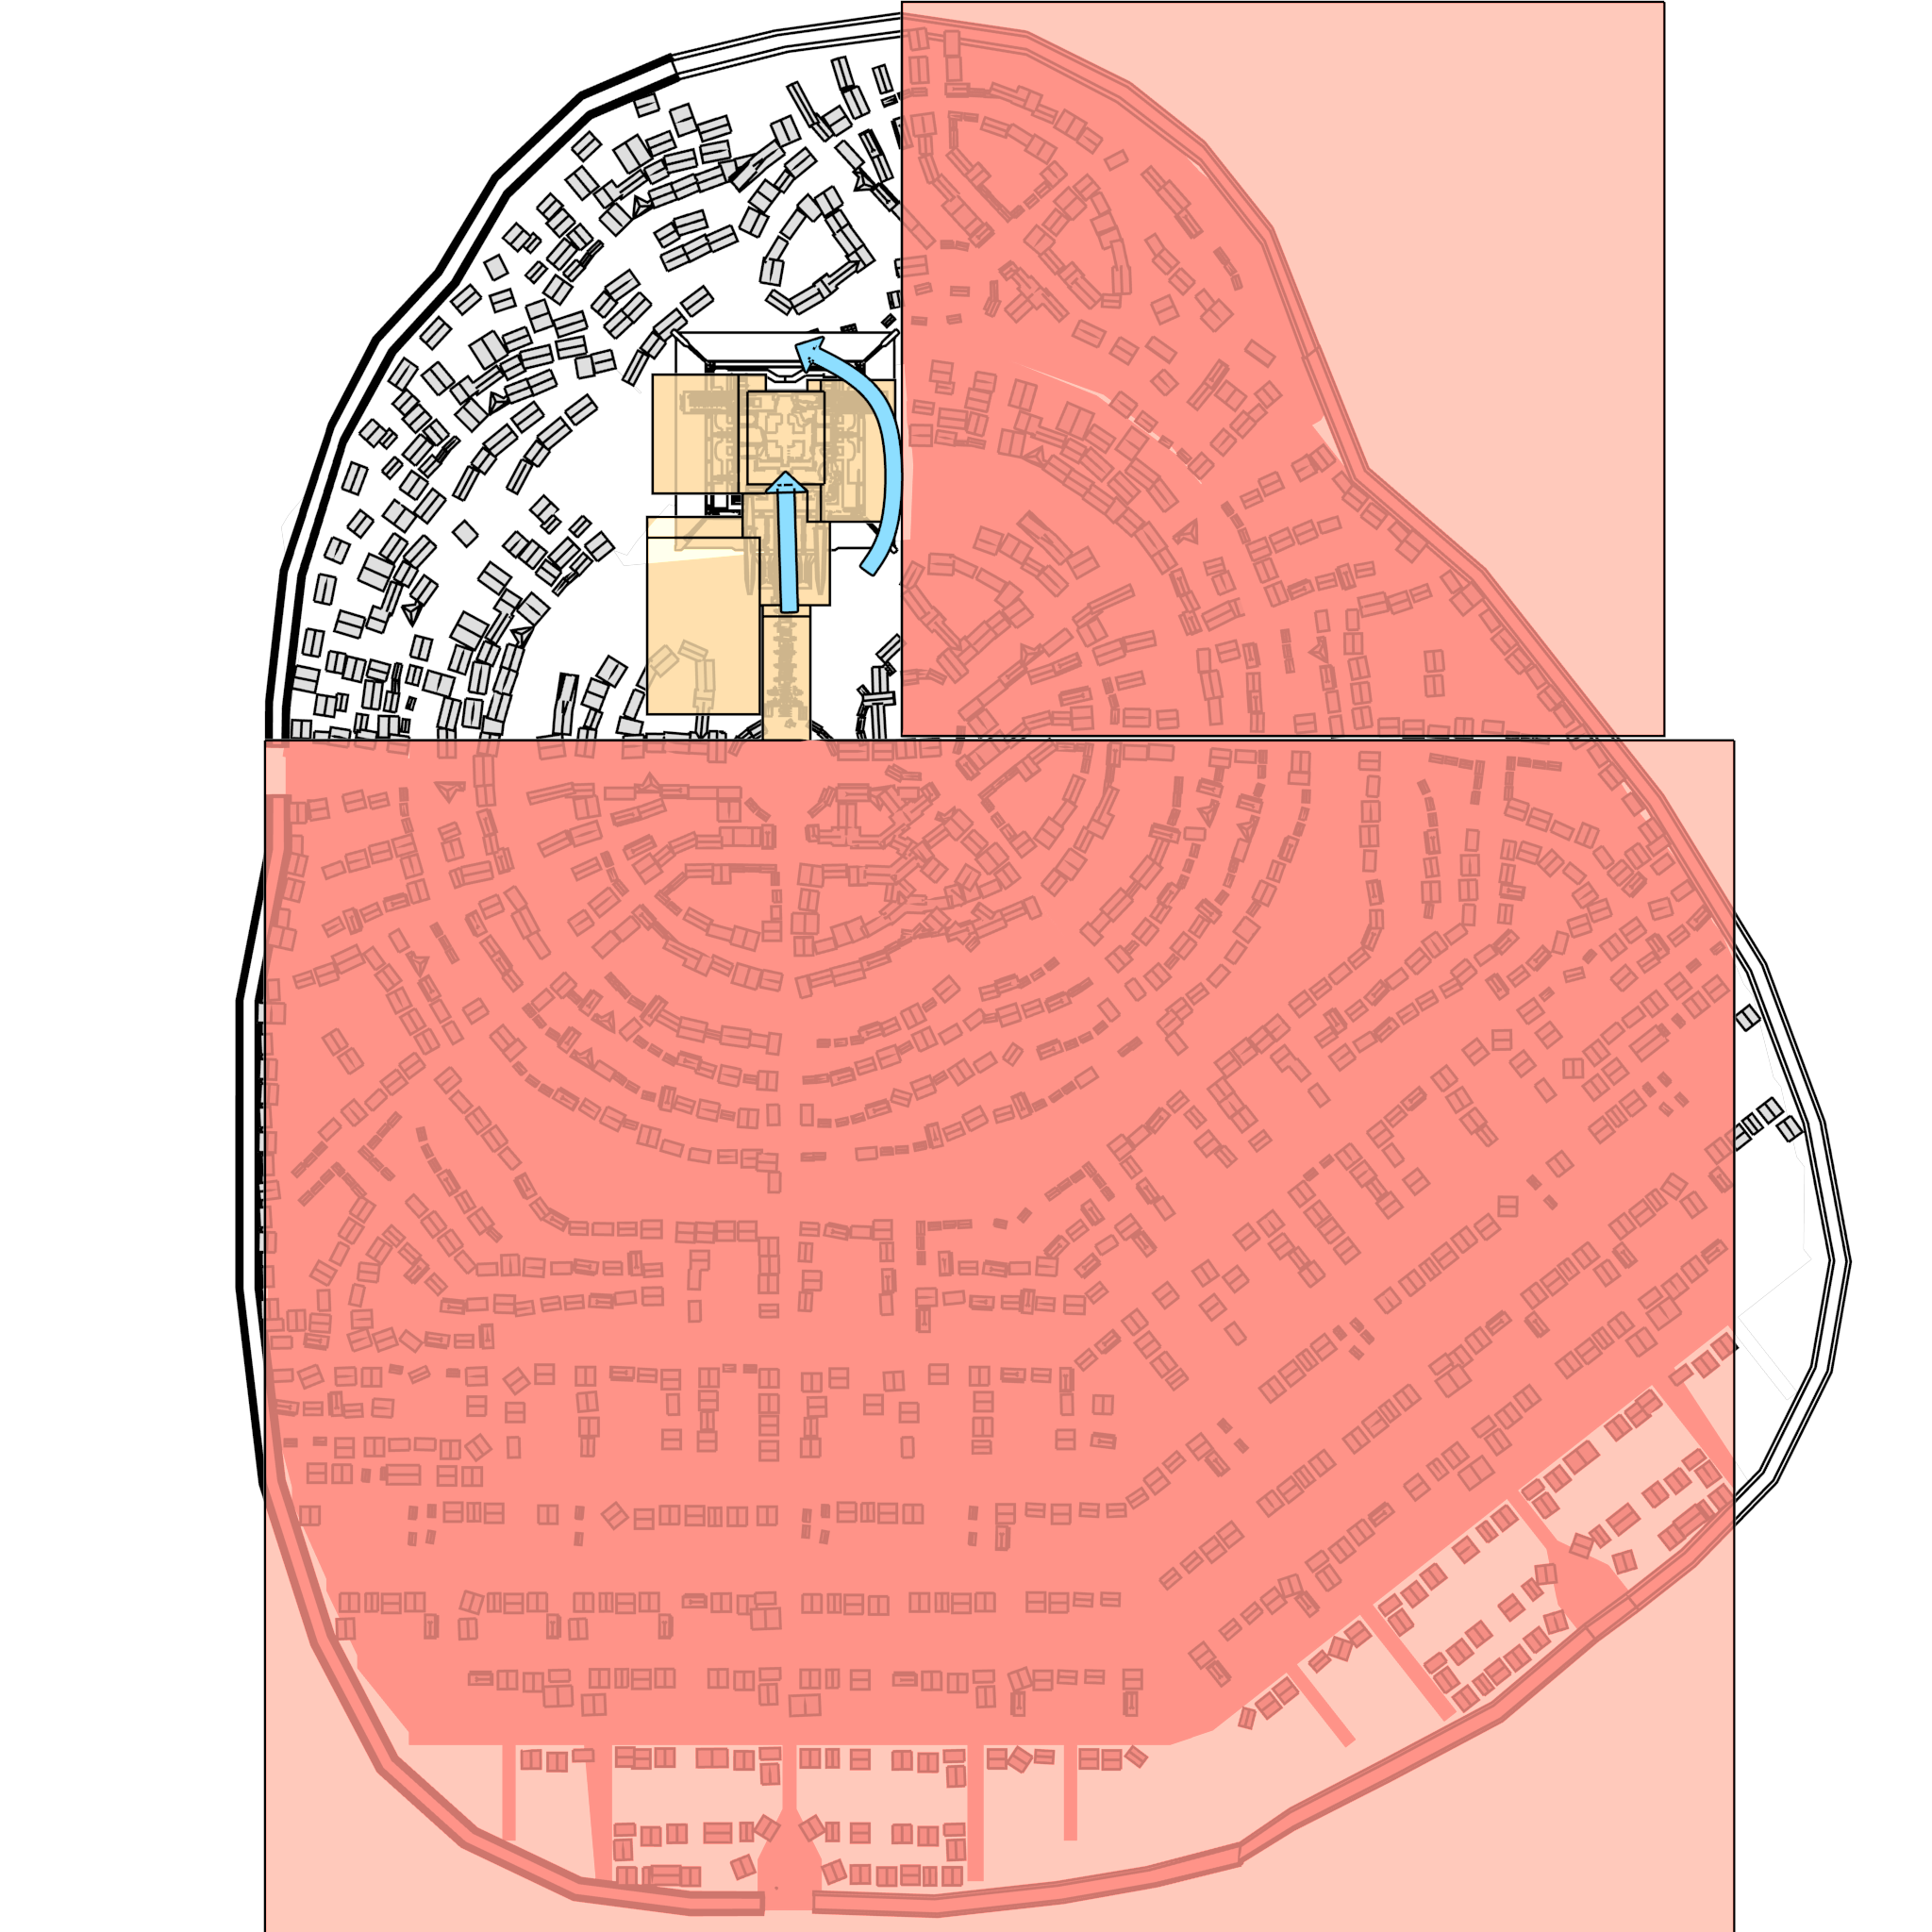
\includegraphics[width=\textwidth]{./img/raw/test-suite-ziggurat-map.png}};
    \node[inner sep=0pt] (map) at (0.05\textwidth, 0.1\textwidth) 
         {
\includegraphics[width=\textwidth]{./img/raw/test-suite-ziggurat-map-size.png}};
    \node (l3) at (-0.3\textwidth, 0.421\textwidth) {$10$ eenheden};
  \end{tikzpicture}
  \caption{Een overzicht van de Ziggoerat stadsscene.}
  \label{fig:test-suite-ziggurat-map}
\end{figure}

